\section{Model III: Genre Comparison, Distinction and Change}\label{sec:model-genre}

This section addresses the genre-level questions of Problem~C: comparing
similarities (and, with Model~I, influences) within and between genres;
asking what distinguishes a genre; asking how genres change over time; and
asking whether some genres are related to others. Throughout we keep a
single genre representation so that the subsections stay coherent.

\subsection{Genre Representation: Katz-Weighted Feature Centroids}\label{subsec:q3-centroids}

Let \(\tilde{\mathbf{x}}_i\in\mathbb{R}^{p}\) be the globally \(z\)-scored
Spotify feature vector of artist \(i\) (the same \(p=11\) coordinates and
standardization as Model~II), and let \(K_i\) be the outgoing Katz score
from Model~I. For each official main genre \(g\) we define the
\emph{influence-weighted} genre vector
\begin{equation}\label{eq:cg}
\mathbf{c}_g
=\frac{\sum_{i:\,\mathcal{G}(i)=g} K_i\,\tilde{\mathbf{x}}_i}
      {\sum_{i:\,\mathcal{G}(i)=g} K_i}.
\end{equation}
Artists who transmit influence more broadly therefore pull the genre
profile more strongly. An equal-weight centroid is retained only as a
robustness check (off-diagonal correlation of the two distance matrices
\(\approx 0.73\)). After joining Model~II features to Model~I scores we
obtain \(n=5599\) artists across 19 genres.

Between-genre discrepancy is the Euclidean distance
\(d_{gh}=\|\mathbf{c}_g-\mathbf{c}_h\|_2\), with bounded similarity
\(s_{gh}=1/(1+d_{gh})\). Within-genre cohesion is the (Katz-weighted) mean
distance of artists in \(g\) to \(\mathbf{c}_g\). Empirically the mean
within-genre cohesion is \(2.92\), below the mean between-genre centroid
distance \(3.79\): genres remain separated at the aggregate level even
after influence weighting. The closest pairs are Blues--R\&B
(\(d\approx 0.76\)), Blues--Country (\(0.78\)) and Latin--R\&B (\(0.86\));
the farthest involve Avant-Garde against Comedy/Spoken, Children's and
Country (\(d>8\)).

\begin{figure}[t]
\centering
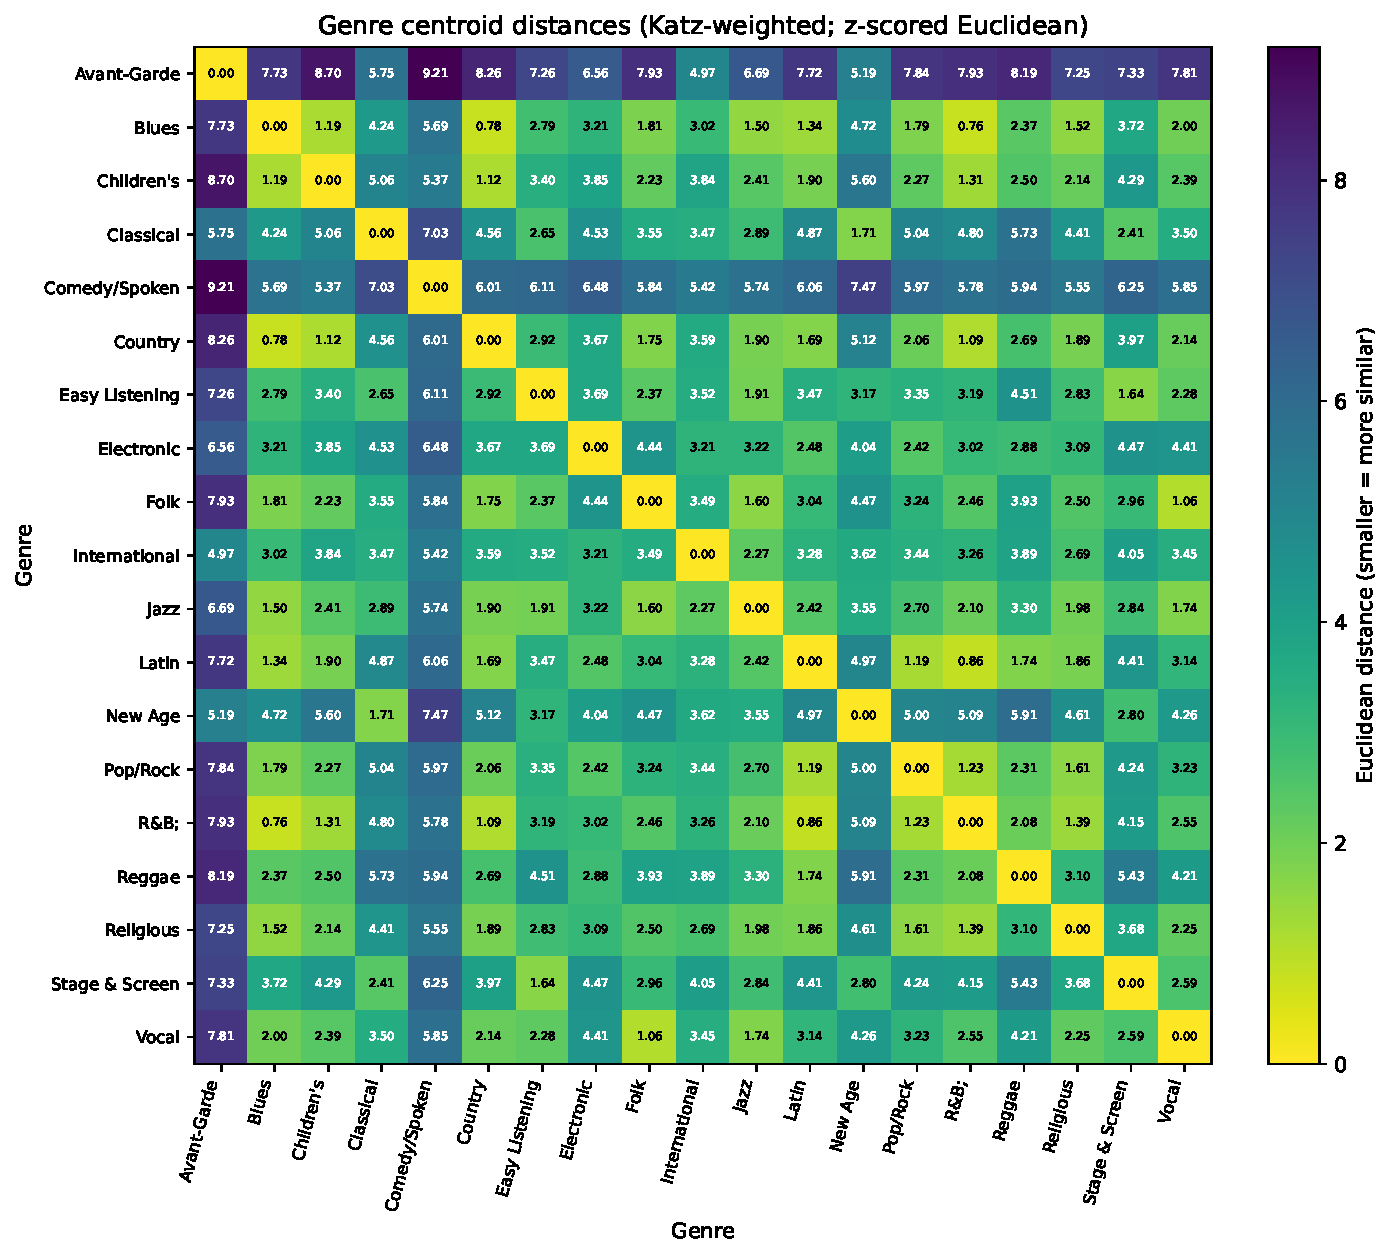
\includegraphics[width=0.65\textwidth]{heatmap_genre_distances_katz.pdf}
\caption{Pairwise Euclidean distances between Katz-weighted genre
centroids \(\mathbf{c}_g\) (smaller $=$ more similar).}
\label{fig:q3-genre-dist}
\end{figure}

\subsection{What Distinguishes a Genre?}\label{subsec:q3-distinguish}

We do \emph{not} assign each genre a unique exclusive feature: with
\(p=11\) features and 19 genres that would be neither feasible nor
meaningful. Instead we read the \emph{same} vectors \(\mathbf{c}_g\). In
\(z\)-space each coordinate of \(\mathbf{c}_g\) is already a signed
deviation from the all-artist mean, so a genre is distinguished by its
\emph{profile}---which coordinates are high or low together.
The most discriminating coordinates globally are
\texttt{duration\_ms}, \texttt{speechiness}, \texttt{instrumentalness}
and \texttt{valence}. Extreme profiles include Avant-Garde (very long
duration), Comedy/Spoken (very high speechiness) and Classical / New~Age
(high instrumentalness and acousticness, low loudness/energy). By
contrast Pop/Rock, Latin and R\&B lie closest to the global mean
(\(\|\mathbf{c}_g\|_2\) small), consistent with coarse, heterogeneous
labels. Even near neighbours remain separable by a few coordinates: e.g.\
Blues versus R\&B differ mainly in loudness, energy and acousticness.

\subsection{How Genre Similarity Changes over Time}\label{subsec:q3-sim-time}

To study change we keep the definition~\eqref{eq:cg} but index it by the
artist's active-start decade \(t\) (Assumption~A2): \(\mathbf{c}_g(t)\) is
formed from artists of genre \(g\) who \emph{began} in decade \(t\), still
weighted by the Model~I Katz score, in the same global \(z\)-space. A
genre enters decade \(t\) only if at least five such artists are present.
We treat 1950--2000 as the main window; the 1930s and especially the
2010s are sparse (only four genres meet the threshold in the 2010s).

\begin{figure}[t]
\centering
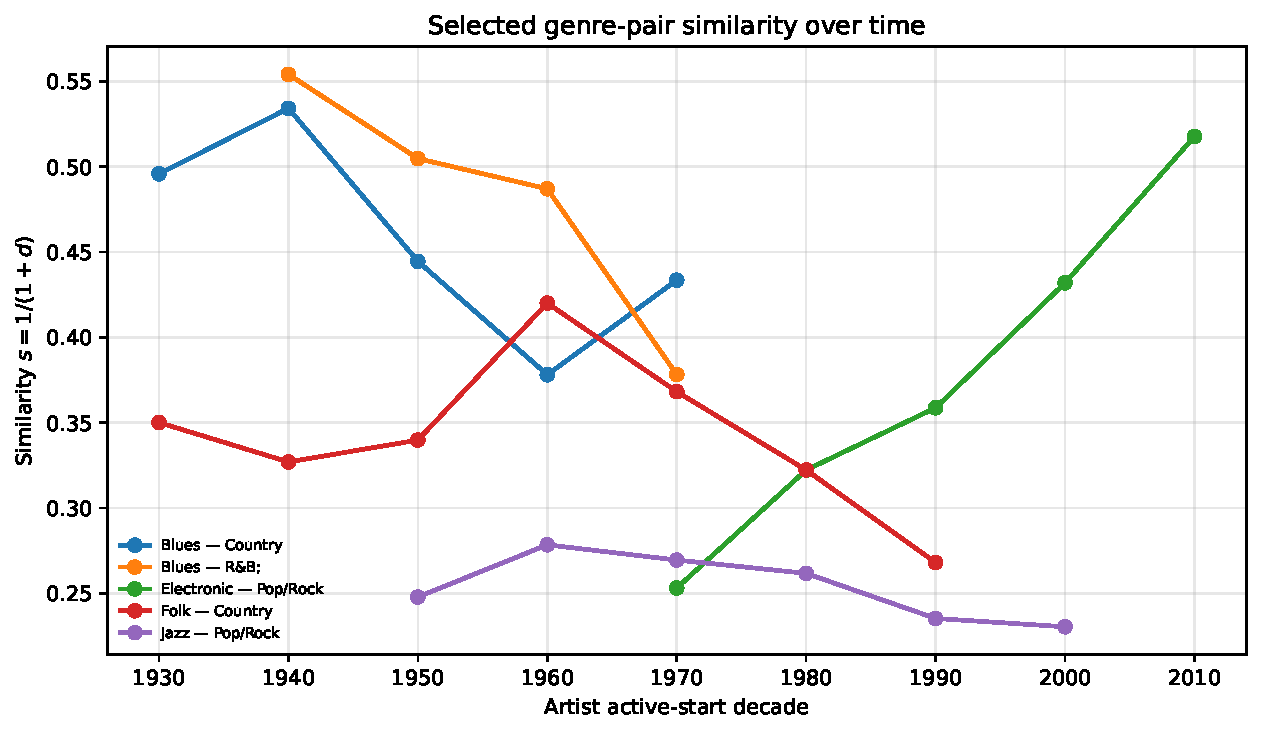
\includegraphics[width=0.65\textwidth]{genre_pair_similarity_over_time.pdf}
\caption{Similarity \(s=1/(1+d)\) for selected genre pairs over decades.
Electronic--Pop/Rock becomes more similar; Blues--R\&B and Folk--Country
trend slightly apart where both are observed.}
\label{fig:q3-pair-time}
\end{figure}

Mean between-genre distance rises from about \(3.16\) (1950s) to about
\(4.55\) (2000s): later cohorts are, on average, more sonically separated.
Pairwise trajectories are heterogeneous---Electronic and Pop/Rock move
closer (\(\Delta s\approx +0.18\) from the 1970s to the 2000s), while
Blues--R\&B similarity falls over the decades in which both are observed.
Self-drift \(\|\mathbf{c}_g(t)-\mathbf{c}_g\|\) is largest for
Comedy/Spoken, International and Classical, indicating that their
decade-specific weighted profiles move farthest from the static
\(\mathbf{c}_g\).

\subsection{How Genre Influence Changes over Time}\label{subsec:q3-inf-time}

% ---------------------------------------------------------------------------
% PLACEHOLDER — teammate (Model I / network side); filled via
% model3_s74_s75_supplement.tex when that file is \input from main.
% ---------------------------------------------------------------------------
\textbf{[Teammate TODO --- genre influence over time.]}
Using the directed network of Model~I, quantify how \emph{influence}
among genres evolves by active-start decade (or edge-endpoint decade):
e.g.\ cross-genre edge counts / share, genre-level outgoing Katz mass, and
export from one genre into another. Place the resulting time series next
to \cref{fig:q3-pair-time} and discuss where sonic similarity and
reported influence move together or diverge.
% End placeholder.

\subsection{Are Some Genres Related to Others?}\label{subsec:q3-related}

% ---------------------------------------------------------------------------
% PLACEHOLDER — synthesize similarity (done) with influence (teammate)
% Can reuse fig:q3-genre-dist and closest/farthest pairs; add a joint
% scatter or two-panel figure: similarity vs cross-genre influence.
% ---------------------------------------------------------------------------
\textbf{[TODO --- relatedness synthesis.]}
The distance matrix in \cref{fig:q3-genre-dist} already supplies a sonic
relatedness graph (Blues--R\&B--Country--Latin as a close cluster;
Avant-Garde as an outlier). Complete this subsection by combining that
picture with Model~I cross-genre influence: genres may be (i)~sonically
close and strongly cross-linked, (ii)~sonically close but weakly linked,
or (iii)~sonically far yet heavily cross-influencing. A short taxonomy of
a few genre pairs under these three regimes answers whether ``related''
should mean sound-alike, citation-linked, or both.
% End placeholder.
